\section{Problem 2}

\lstinputlisting{p2.py}
We set out to make initial density fields based off of the power spectrum,
\begin{equation}
  P(k) = k^n,
\end{equation}
where $n$ is $-1, -2, -3$. Essentially, we setup the indices for the Fast
Fourier Transform (FFT) as described in the slides. We define the function
for the power spectrum, use our rng to make random numbers, and finally
perform the FFT on each field. Figures are plotted below.

\begin{figure}[h!]
    \centering
    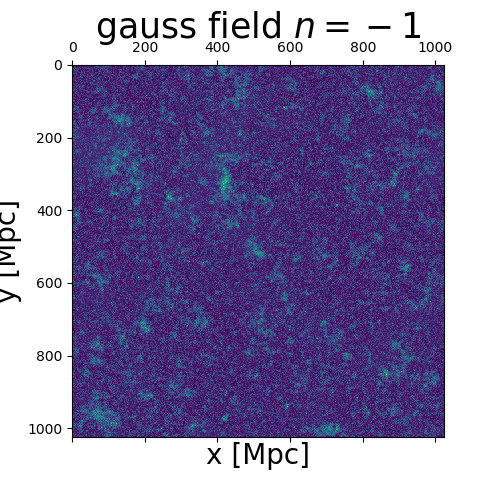
\includegraphics[width=0.9\linewidth]{./plots/gauss_field_-1.png}
    \caption{Gaussian field for $n=-1$.}
    \label{gf1}
\end{figure}
The initial field in \autoref{gf1} looks roughly what we expect.
Admittedly, I am unsure exactly what is expected, but as the handout
explains, dispersion is dependent on $n$. In \autoref{gf2} we can see
the dispersion causes a bit more ``clumpiness'' (that is, high-density
pockets). In \autoref{gf3}, we see an even higher contrast between
the low-high density regions. (Sorry, my colorbar was not working! It's 
viridis colormap, though.)
\begin{figure}[h!]
    \centering
    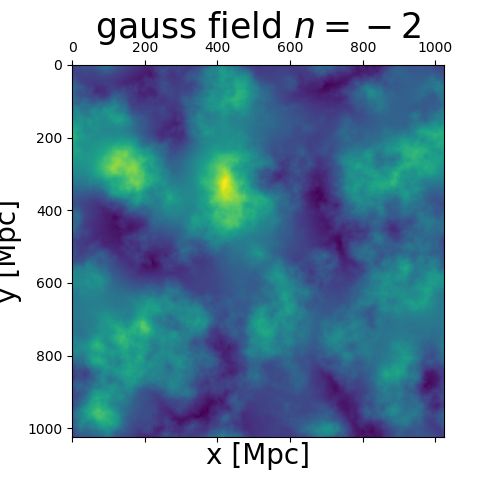
\includegraphics[width=0.9\linewidth]{./plots/gauss_field_-2.png}
    \caption{Gaussian field for $n=-2$.}
    \label{gf2}
\end{figure}
However, in \autoref{gf3} it is clear something is wrong. The physical
distances are not changing as a function of $n$. As $P_k$ changes from
$n=-1$ to $n=-2$ for example, the maximum and minimum k values should increase
from $n=-1$ to $n=-2$. The physical distances should be larger as well.
Given time constraints, I gave up and left the plots as is. I assume 
it has a $2$-fold issue: my rng and perhaps the amplitudes are not actually
changing as expected.
\begin{figure}[h!]
    \centering
    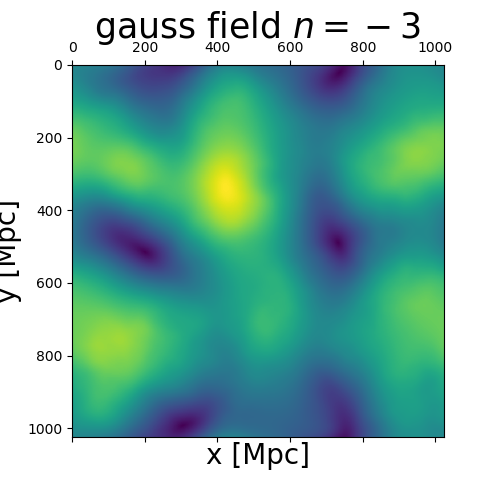
\includegraphics[width=0.9\linewidth]{./plots/gauss_field_-3.png}
    \caption{Gaussian field for $n=-3$.}
    \label{gf3}
\end{figure}

